\section{mul-biguint}
\label{mul-biguint}

\begin{enumerate}
    \item target
        \begin{itemize}
            \item implenment the multiplication of two biguints
        \end{itemize}
    \item constraints-logic
        \begin{itemize}
            \item equation for gate.
            \item sumcheck between ouptput and limbs
            \item rangecheck for limbs
        \end{itemize}
    \item mul-process layout
        \begin{figure}[!ht]
            \centering
            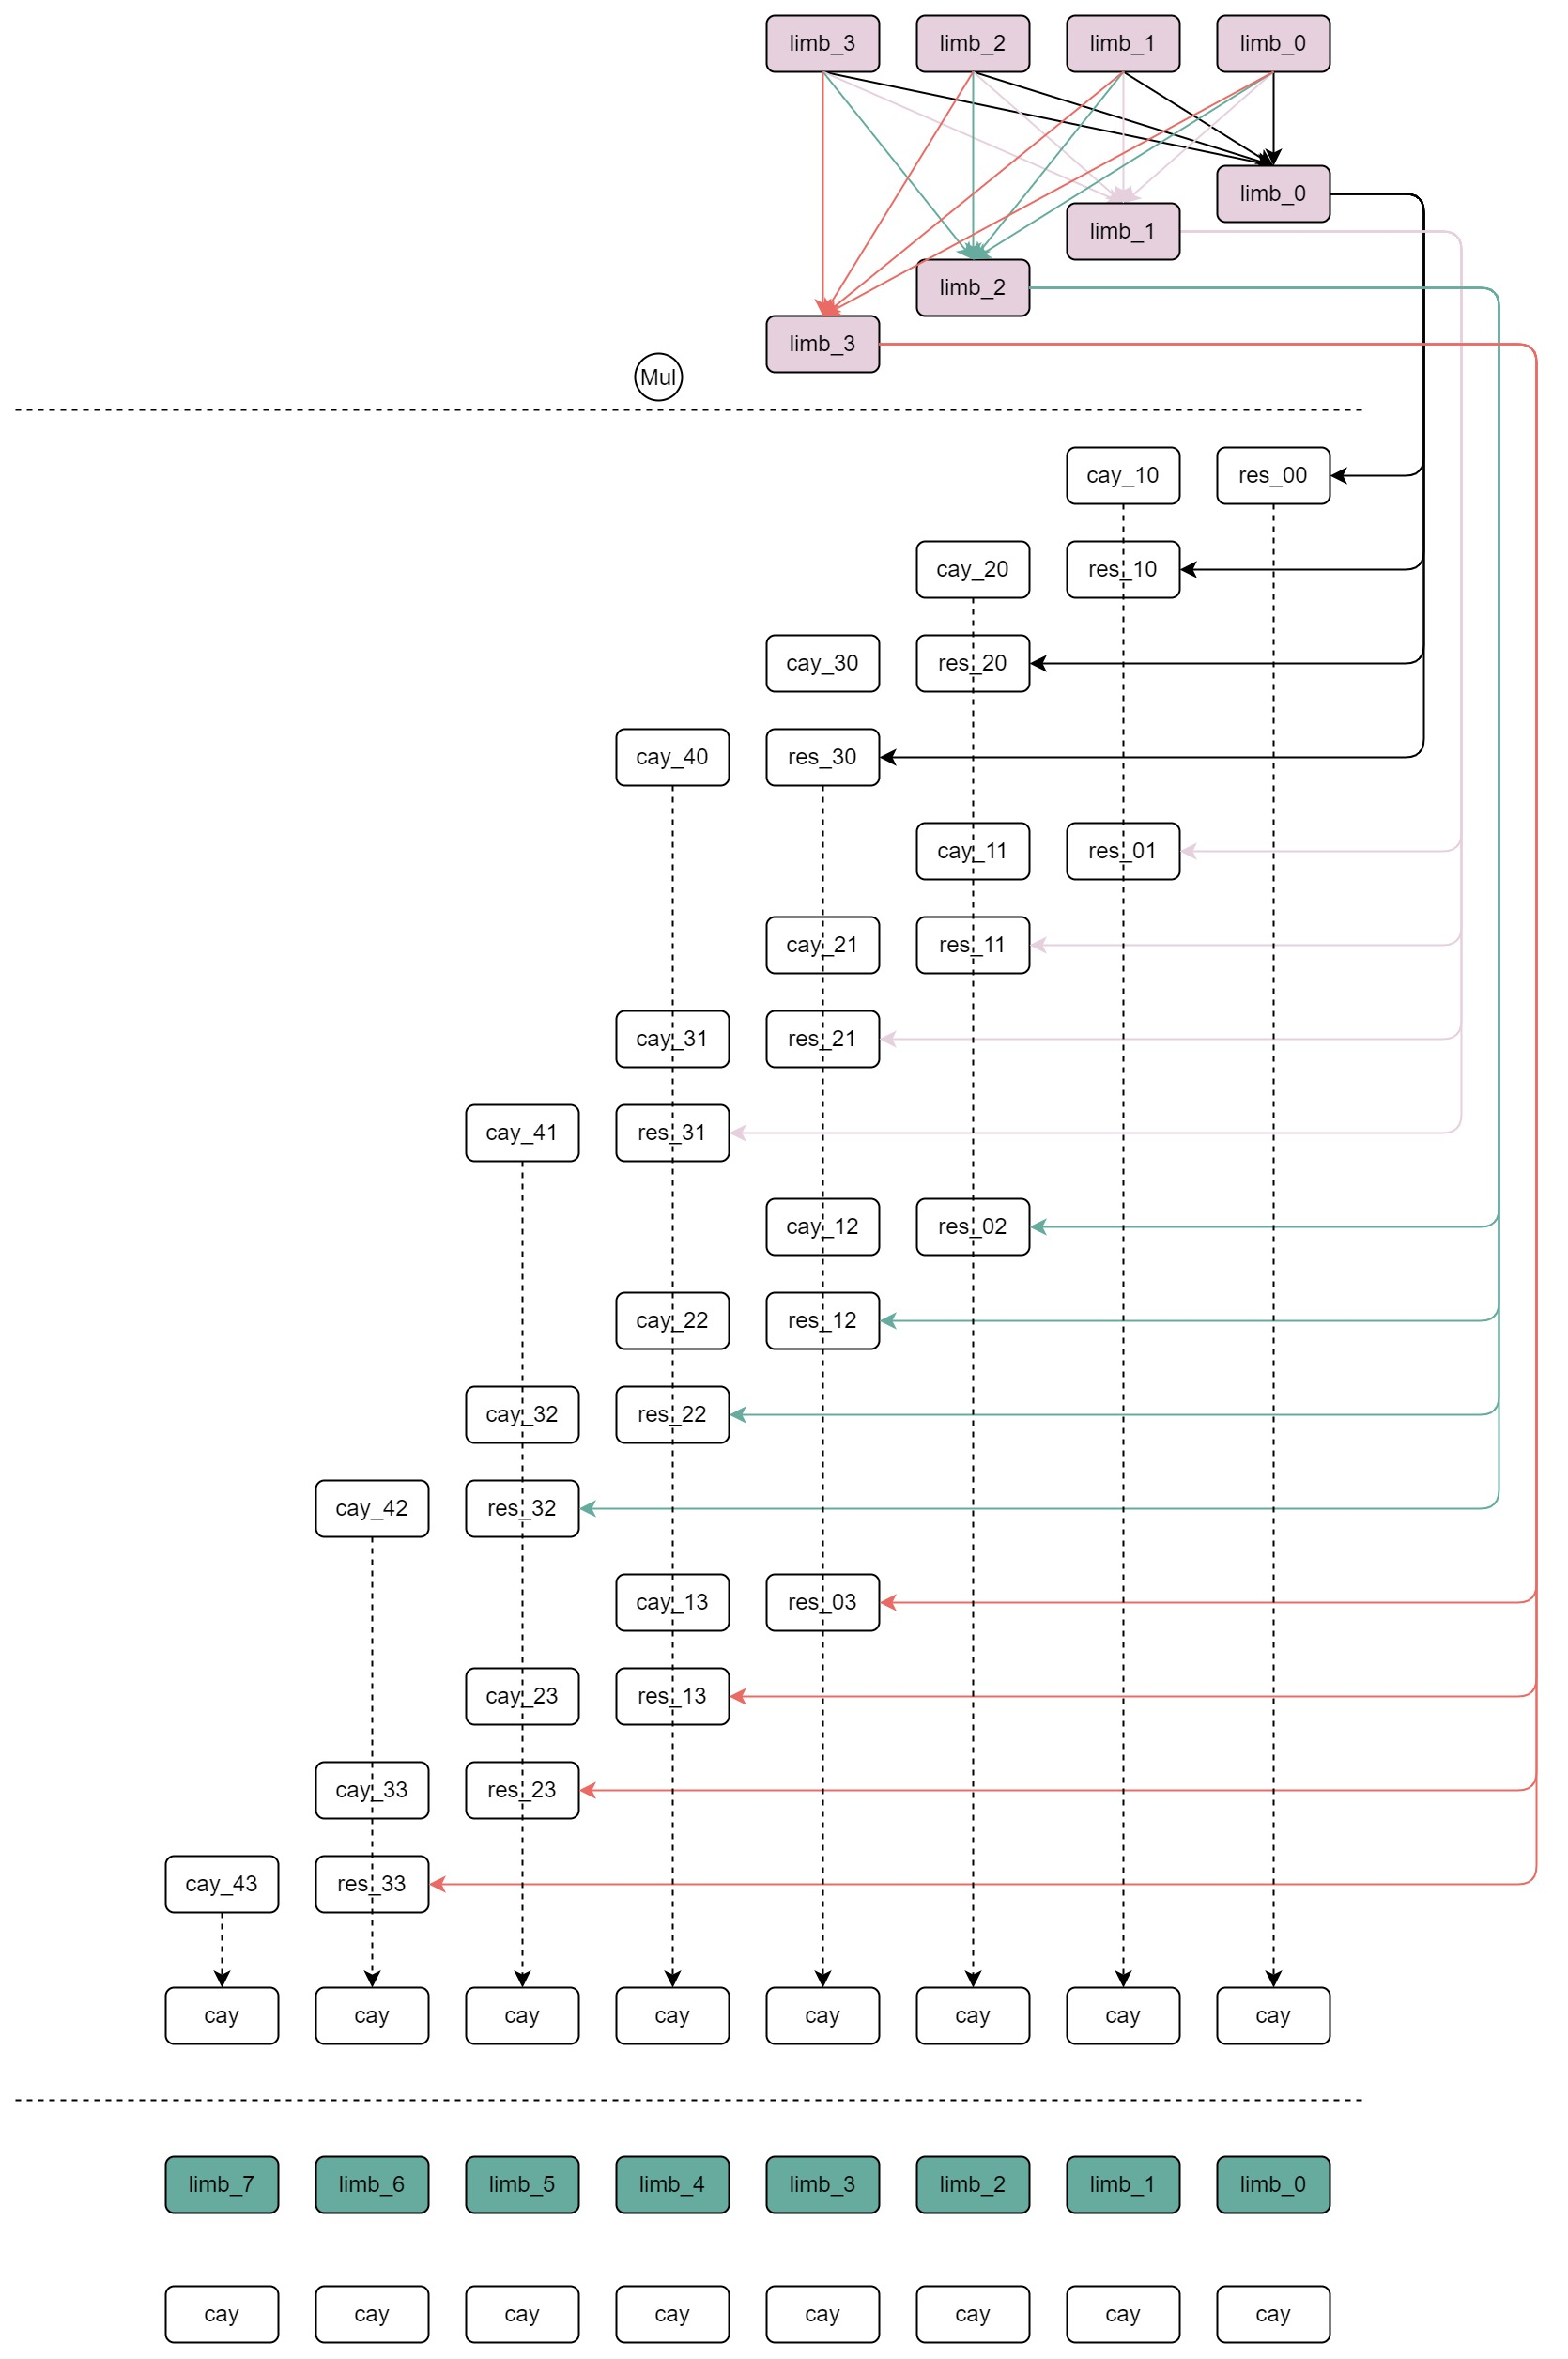
\includegraphics[width=0.8\textwidth]{mul-biguint-layout.jpg}
            \caption{Mul-biguint layout.jpg}
            \label{fig:mul-biguint-layout.jpg}
        \end{figure}

    \item trace layout
        \begin{figure}[!ht]
            \centering
            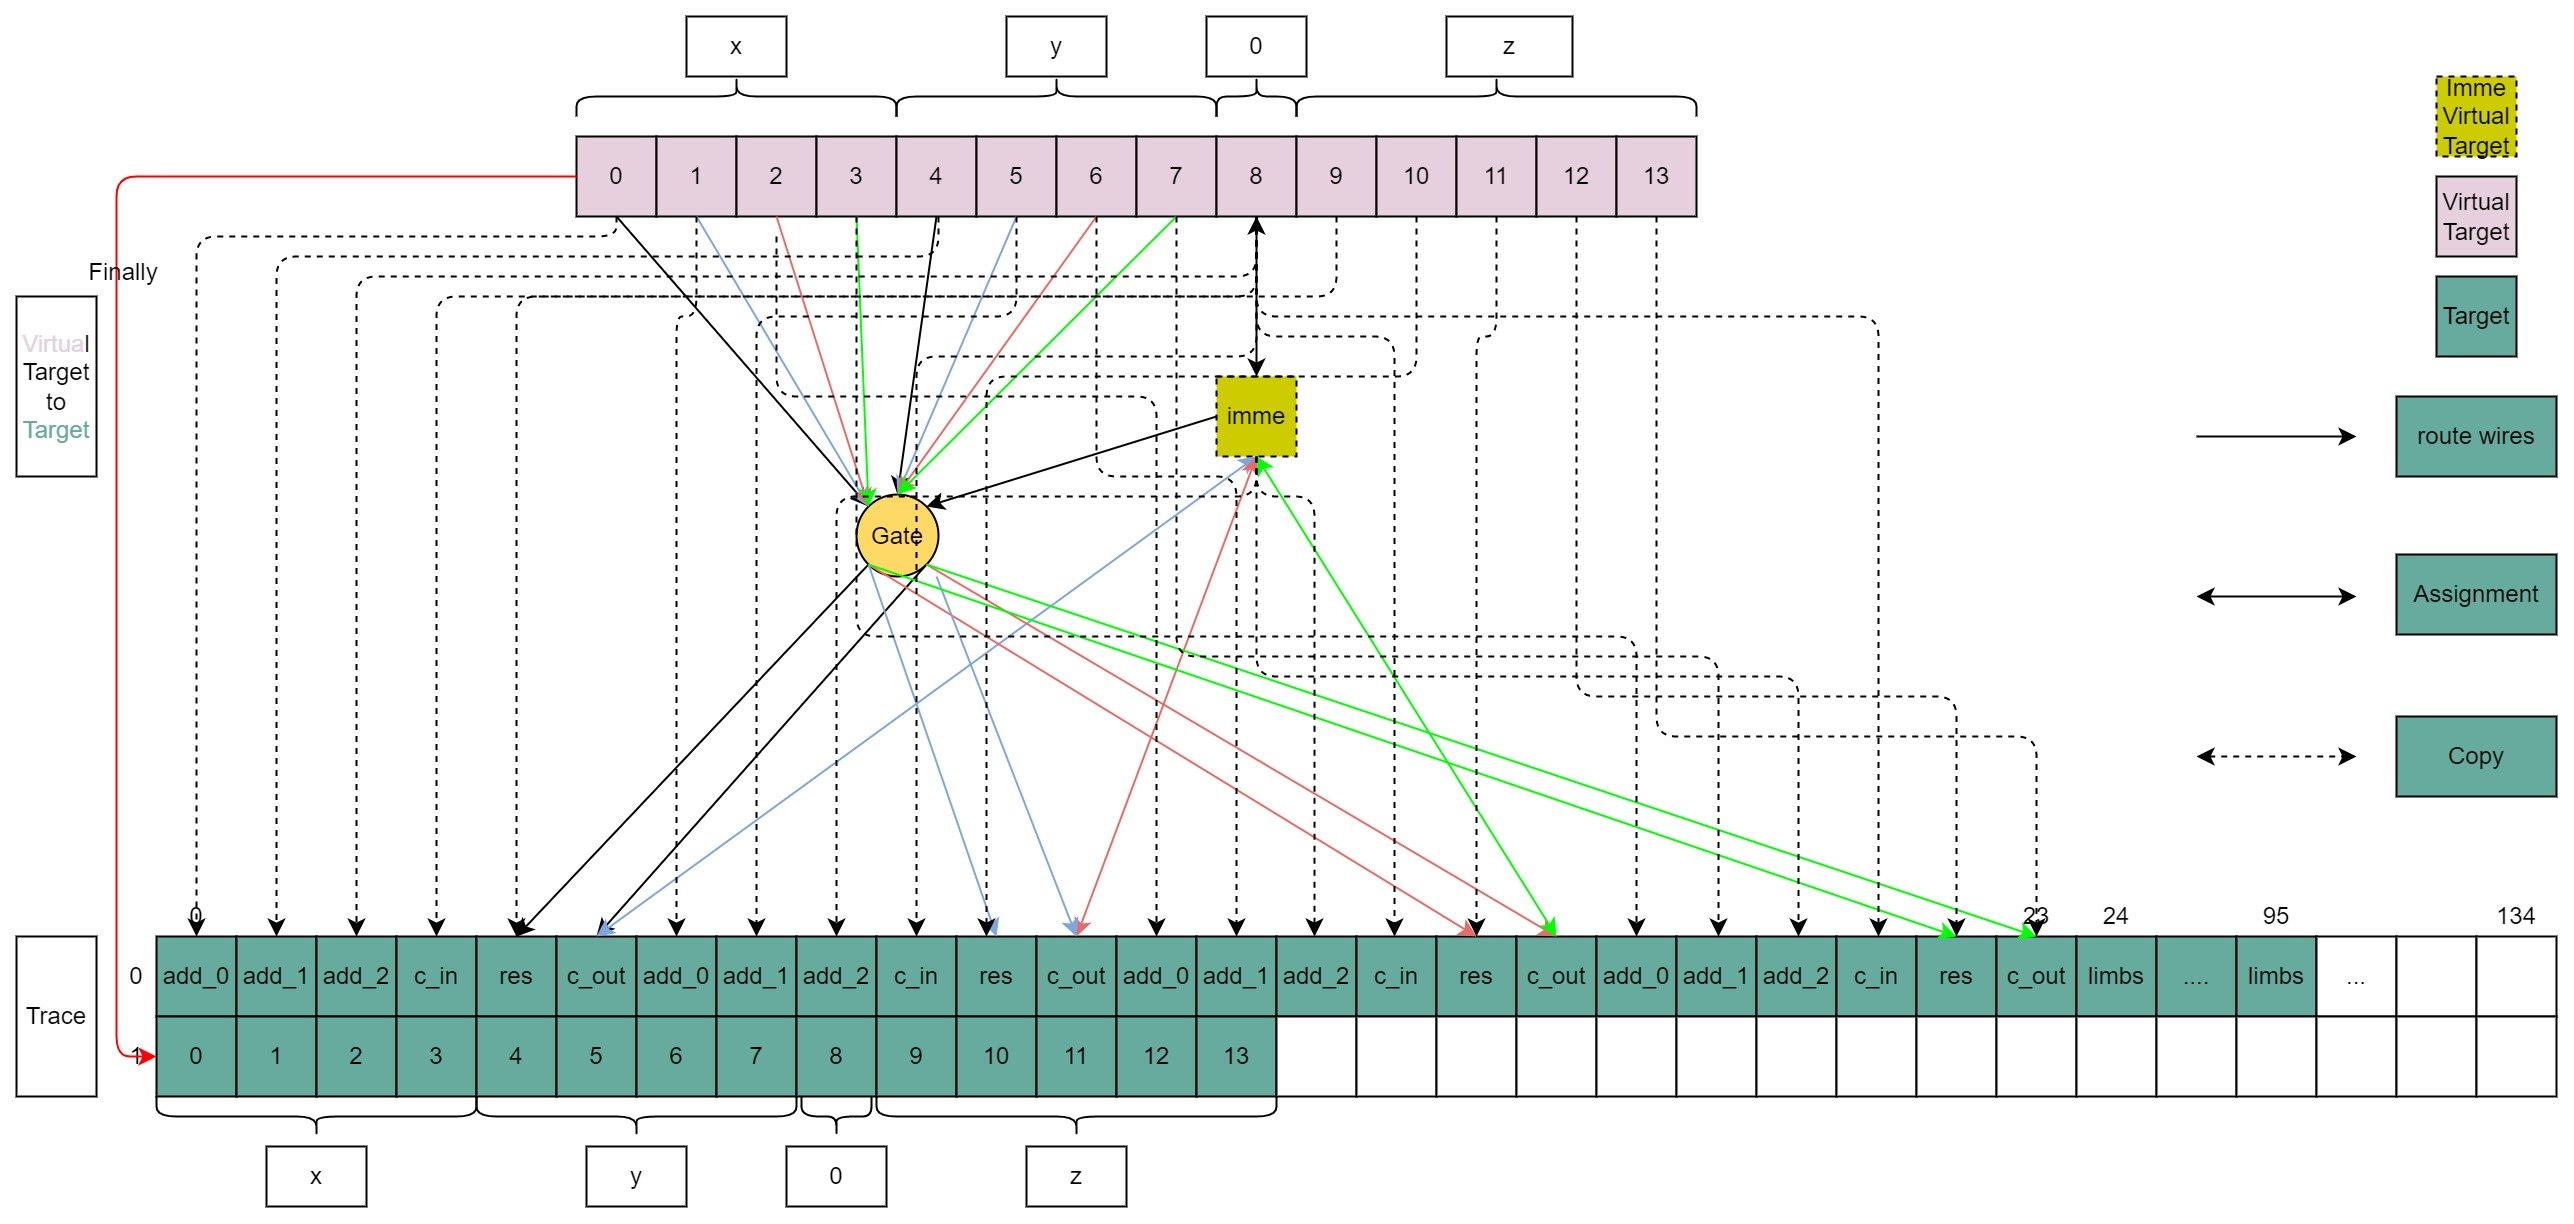
\includegraphics[width=0.8\textwidth]{add-biguint-trace-layout.jpg}
            \caption{Add-biguint trace layout}
            \label{fig:add-biguint-trace-layout}
        \end{figure}
    
    \item constraints-info and costs
        \begin{itemize}
            \item constraints-num: 5 * (3 + 32 / 2 + 4 / 2) = 105
            \item copy-constraints: 4 * 5 + 6 = 26
            \item max-degree: 4
            \item wires-num: 5 * (6 + 16 + 2) = 120
        \end{itemize}

    \item questions
        \begin{itemize}
            \item why not make rangecheck constraint for inputs?
            \item why not make copy constraint between cur-c-in and last-c-out?
        
        \end{itemize}

\end{enumerate}